\documentclass[10pt,twocolumn]{article}

\usepackage{oxycomps}
\bibliography{references}

\pdfinfo{
    /Title (SpatialDB: A Database for Storing Dense Three-Dimensional Voxel Structures)
    /Author (Nicholas Novak)
}

\title{SpatialDB: A Database for Storing Dense Three-Dimensional Voxel Structures}
\author{Nicholas Novak}
\affiliation{Occidental College}
\email{nnovak@oxy.edu}

\begin{document}

\maketitle

\section{Introduction and Problem Context}

% What my project is
In my senior comprehensive project, I have designed and implemented a database
application that is designed specifically to store complex shapes in ``voxels'',
or three-dimensional pixels.

% Applications of voxels
A voxel\cite{enwiki:1186283262} represents a single point or cube in a
three-dimensional grid, at a variable size. This feature allows them to
approximately model many three-dimensional structures, and to reduce the
computational complexity in analyzing the shape, which has led to many
data-related use cases outside of computer science. For example, to model the
inner workings of the brain, Neuroscientists track oxygen concentration through
neural tissue on a voxel grid as part of fMRI studies\cite{norman2006beyond},
and Movie studios such as DreamWorks use voxel data structures to model light
reflections for visual effects\cite{museth2013vdb}. The output of MRI scans in
hospitals are very high-resolution voxel grids. Most recently, machine learning
models are being trained on the LIDAR data from self-driving
cars\cite{li2020deep} in order to better process their environments. However,
voxels are not often thought of as a way to permanently store three-dimensional shapes, and
existing research focuses mainly on efficiently representing and processing
shapes. My approach models this problem of voxel storage and representation, and
turns it into a problem of database design.

\subsection{Using Minecraft as a Model for a Database}

% The problems with Minecraft
Minecraft\footnote{https://www.minecraft.net/en-us}, released 2009, is a sandbox
game that is played in a world entirely composed of cubic voxels, where the
player has complete freedom to manipulate the world by building, destroying, or
exploring any part of it. I am focusing this database on the requirements of
Minecraft because the game involves some additional challenges that traditional
databases do not consider. Primarily, the world of Minecraft is infinite in the
horizontal $x$ and $z$ axes, but fixed in the $y$ axis, which limits the amount
of information that can be stored by the database at once. The world also
contains a denser voxel grid than in many other applications, meaning that far
more of the blocks in the world are filled than empty.

A game is also a real-time application, which means that any performance issues
will be immediately be present to the user. Most databases can be evaluated on
only their speed, but as the Minecraft server processes new information 20 times
per second, the game has a time budget of 50ms to handle all game logic,
including the storing of data. Less time processing the data in the world means
that more time will be freed up for the game to process other work, although
finishing work earlier will not necessarily be faster for the end user, if it
still under the budget of 50ms. Most databases do not meet this requirement, and
even though they may be faster, their complexity does not mean that they will
always finish operations within this time limit.

These limitations also make Minecraft unable to take advantage of a cache, since
the number of different operations that can be done on the world is infinitely
large, remembering any previous operations will often not be helpful for the
system's performance. Minecraft also provides a good benchmark for the database,
because the unpredictability of players stresses the system's ability to return
results in a variety of settings.

\section{Technical Background}

\subsection{What is a database?}
When I refer to the concept of a database, I am referencing a program that sits
more or less as a ``black box'' between the user and a software application,
storing any data required for the application. In most existing applications,
this is done by a category of databases called ``relational databases'', which
offer a very general-purpose way to store user data that is highly connected.
For instance, a person stored in a relational database would be efficiently
linked to with any of their associated information, such as name or age.

% The model of a database
In database terms, any amount of data added to the database is called a
``write'', data retrieved from the database is called a ``read'', and any
questions asked, such as ``how many people have done this'', are called
``queries''. Developers ask these questions through computer languages, one such
example being Structured Query Language or SQL, which allow
the database to be queried efficiently.

\subsection{Challenges With Existing Databases}

% Software development and SQL
Most software engineering projects start with a simple front-end and back-end,
typically implemented with some sort of Model-View-Controller architecture, and
connected to a relational SQL database \cite{sqliteOnlyDatabase}. This idea was
popularized by frameworks such as Ruby on Rails and Django, where the model was
most often modeled by structures within the database. This framework allowed
software developers to not have to worry about inner workings of the database,
and focus on writing business logic. This is how many start-ups were built, such
as GitHub \cite{githubSingleSQL}, who recently moved off its single SQL database
after 13 years, citing performance issues.

% Challenges with working with SQL: Performance
Using a single SQL-speaking database can be a significant advantage development
speed, but the database can have some issues keeping up with the demands of the
application as the performance requirements expand.
% Caching
As soon as this happens, companies typically put smaller caching applications in
front of their database, such as \verb|Redis|\footnote{https://redis.io/},
\verb|memcached|\cite{nishtala2013scaling}, or \verb|TAO| \cite{bronson2013tao},
to allow the application to remember some of the commonly asked questions and
reduce load on the database by not having to do the same work again.

\subsubsection{The Complexity of General-Purpose Databases}
% What is being done about this
Modern SQL databases are also very complex. Three of the most popular SQL
databases, PostreSQL, MySQL and Sqlite have 1.4 million lines
\footnote{https://wiki.postgresql.org/wiki/GSoC\_2018, in reference to the
text ``PostgreSQL is over 1.3M lines of code and some of the code paths can be
tricky to reach.''} of code, 2.9 million lines
\footnote{https://www.openhub.net/p/mysql}, and 150,000 lines
\footnote{https://www.sqlite.org/testing.html} respectively.

% Why are databases inefficient?
Why are databases so complex? Most of the reason for the complexity is that
because these database systems so general-purpose, they cannot assume anything
about the data stored in them. For the database, finding an efficient plan to
answer each query is a known NP-hard problem\cite{chatterji2002complexity}, and
to keep itself fast, the database must construct this plan with a complex set of
approximations, based on the assumptions that it can make, which leads to
ever-evolving complexity.

% Impossible to maintain
With this complexity, it is impossible for a single person to understand the
complete inner workings of a database. Thus, the problem of the company's
database often becomes a dedicated person in companies that can afford it, or
become entire teams of engineers at larger organizations such as
Google\cite{googlePerfTeam}.

% Intro to special-purpose databases
What happens in the larger companies that can afford more engineering time, and
have a specific problem that they cannot solve with a traditional database?
Typically, this leads to the creation of special-purpose database solutions. For
instance, the global scale of iCloud and Apple's cloud solutions required them
to create FoundationDB\cite{zhou2021foundationdb}. A different set of challenges
in the Facebook inbox led to the creation of Apache
Cassandra\cite{lakshman2010cassandra}, which is optimized to allow for many
emails to be received, at the expense of search speed, which is done far less
frequently.

\subsubsection{The Special-Purpose Database}

Limiting a database's design to a specific use-case can make the development
process much simpler, to the point where it can be done by a single person, and
can offer higher performance. The first question that needs to be asked is
whether the application is \textit{write-heavy} or \textit{read-heavy}.
Read-heavy applications occur often in web development, and most social media
platforms have far more users reading the content, than writing new content for
the platform. In contrast, write-heavy applications are often seen in analytics
workloads, where data is written from many sources, and analyzed infrequently by
users.

My application has a relatively even write and read balance, and I evaluated
three different storage data structures before choosing to implement my own

% Special-purpose databases
Recently, companies such as Tigerbeetle\cite{tigerbeetleDesign} have taken this
domain-driven approach to database design even further, while designing a
database from the ground up to do financial accounting, which outperforms a
reference MySQL implementation at 76 accounting transactions per second, to
1,757 transactions per second \cite{tigerbeetlePerf}. This highly specialized
and domain-specific approach to creating databases is what my project is going
to be based on, to create a database around the challenges that the game
Minecraft has.

\subsubsection{Key-Value Databases}

One of the main architectures that I considered for my project is a design
called a key-value store\cite{kvdatabase}, which would store the relationship of
a single voxel to its value. Many other voxel databases use this method to
achieve constant-time operations on retrieving points, which means that
regardless of the size of the dataset, the database will always be able to
return a result in the same amount of time. This structures is behind many of
the high-performance caches that are commonly used to speed up web applications,
such as Redis and RocksDB\cite{dong2021rocksdb}. In order to provide high speeds
for this data, the key-value mappings are usually stored in main memory, which
is far more expensive and limited than the system's disk drive, but offers
a speed advantage of several orders of magnitude\cite{latencyKnow}.

\section{Prior Work}

\subsection{Voxels for Efficient Computation}

Most existing literature on the topic of using voxels to store shapes focuses on
the application of the voxel grid for efficient computation. Since voxel points
are completely independent of each other, this allows for efficient parallel
processors, which are increasingly more common on consumer hardware, to take
advantage of this speedup. In VDB\cite{museth2013vdb} Museth demonstrates that
by modeling a sparse voxel grid in different resolutions, a computer cluster can
efficiently approximate a physical structures such as a cloud, in order to
calculate expensive lighting operations.
% Parallel processing on voxels
Williams\cite{williams1992voxel} expands upon the uses of a voxel database to
model graph and mesh-based problems. Taking advantage of the parallelism in the
grid, many problems can be reframed in the representation of voxels, and solve
those problems far more efficiently. This model however, assumes that every
voxel is stored in shared memory, making this process only viable to solve
problems that can be modeled on one machine, and are far more computationally
expensive, rather than data-intensive.

\subsection{Storing Large Voxel Data Sets}

Another approach to the problem of storing voxel data is the distributed
approach in Gorte et. al. \cite{gorte2023analysis}. Since memory is limited
within one computer, this workload can be split up between many servers, which
allows very large datasets to be worked on by a single workstation through an
API. This method keeps many of the same performance considerations, but also
assumes that the voxel data is not very dense, and uses a three-dimensional
data structure called an octree, which allows the user to change the resolution
of the data that they are working on. In the paper, Gorte acknowledges the need
to split large datasets up into smaller regions, which is similar to the concept
of ``chunks'' in my implementation.

\subsection{Chunk Systems in Other Games}

The decision to choose chunks to represent game data has many justifications. As
\cite{gorte2023analysis} mentions, an infinite grid of voxels needs to be broken
up in a way where applications can store data in an efficient way, and many
other games converge on this same implementation. Another voxel-based game,
Veloren\cite{https://veloren.net} uses the same chunk-based system, although
differs in its storage method. The game switches between several different
storage implementations in each chunk, depending on how dense or sparse the voxel
data within the chunk is. For sparser data, the game stores block information in
a simple key-value hash map. As the number of voxels increase, the game further
breaks this information up, and creates several smaller sections within the
chunk. Finally, for very dense data, the game stores a compressed version using
Zlib compression\cite{veloren32}. This gives many options for data compression
in my database, but also shows how the database can be adapted to store sparser
structures more efficiently if the focus of the project ever needs to change.
Since this game is not based on Minecraft, but an independent project named cube
world, the game comes up with a similar data structure, and shows the
performance considerations for using such a structure. The benchmarks that they
show suggest about an order-of-magnitude improvement over using a key-value
store.

\subsection{Previous Special-Purpose Databases}

The design of my database was also inspired by the LSM tree and data-driven
designs of Tigerbeetle\cite{tigerbeetleDesign}, which is also able to handle
concurrent operations on the same design. Another database,
CockroachDB\footnote{https://www.cockroachlabs.com/product/}, uses a key-value
mapping backend to store a SQL-like tables and rows. Finally, the design of
caching layers in modern SQL caches such as Noria\cite{gjengset2018noria} show
that it it possible to efficiently remember the complex queries found in SQL,
and replicate these in real-time.

\section{Methods}

\subsection{The Interface for the Database}

For developers to interact with the database, the database is implemented as a
library, and the database provides a simple application programming interface to
read and write data, consisting of the following operations. The performance
considerations for each of these operations can be found in the methods section
below.

\begin{itemize}
  \item Read a single block
  \item Write a single block
  \item Change a range of blocks
  \item Read a pre-defined ``chunk'' of blocks
\end{itemize}

\subsection{Reading and Writing a Single Voxel}

The process of updating the data for a single point in the world starts with the
voxel's position. Because the world is infinite on the horizontal $x$ and $z$
axes, this is implemented by a system of ``chunks'', which are fixed-size 16x16
columns of voxels, 256 voxels high. The size of these chunks are chosen so that
they are large enough to be efficiently cached, and many operations can occur
within the same chunk, but not too large to the point where the hundred or so
chunks sent to the user upon joining the world cause a network slowdown. Given a
point's $x$ and $z$ positions, the chunk that that voxel belongs to can be found
with a fast modulus operation, in constant time.

To fetch the data for that chunk, the database needs to read that data from
disk. The database stores this information in combined files that I call ``unity
files'' (shown in figure \ref{fig:unity}), which consist of a single file on disk, but with the encoded data for
each chunk stored as a start index and size, so that the \verb|seek| syscall can
be used to efficiently query this data, while only keeping one file open. This
scheme was used over the previous system of storing chunk files separately,
because the filesystem had a hard time searching through the hundreds of
thousands of chunks in larger worlds. This start position and size are stored in
an auxillary hash map that stores a mapping of every chunk's position to its
metadata within the unity file. This structure uses a minimal amount of memory,
and also allows for a file to be fetched from disk in a constant amount of time
and disk reads.

\begin{figure}
  \centering
  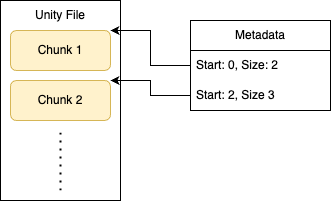
\includegraphics[width=8cm]{unity-file.drawio.png}
  \caption{The Layout of a Unity File}
  \label{fig:unity}
\end{figure}

Each chunk is further divided into sections, in this case each chunk consists of
16 stacked 16x16x16 cubes of voxels, which results in a total of 4096 block
states per section. Using the voxel's $y$ position, the section for a block can
be found with another modulus. Once this is found, a perfect hash function is
used to map the voxel's position to an array index within the section. Again,
both of these steps are done in constant time respectively.

Every section additionally stores a look-up-table, that stores a mapping of a
\textit{palette index} to the state of a block. When the value for the point is
retrieved from the section, the value returned is not the block's state, but
simply an index into this palette. The palette lookup is done in constant time,
and when a new block is added into the section that needs an additional state in
the palette, this value is added in constant time as well. The existence of this
palette supports the efficient operation changing large portions of blocks in
the world.

Once the value of the point is found in the palette, the value can be returned
to the user. A visual diagram of this process can be found in figure
\ref{fig:lookup}.

\begin{figure}
  \centering
  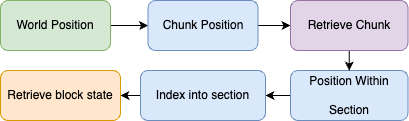
\includegraphics[width=8cm]{block-search.drawio.png}
  \caption{The process of looking up a single block}
  \label{fig:lookup}
\end{figure}

The ability to change a region of blocks is also a common operation within the
database, and which isn't locked to a specific range of chunks. This operation
is implemented as overwriting the palettes for a specific region. By overwriting
every palette index to the same value, every value in the chunk effectively gets
set to the same value. This does however create the need for an additional
``compaction'' step, where the palette is shrunk to remove duplicate values, and
every block within the section must be updated to point to the correct index in
the palette. This compaction is done upon any subsequent writes to the section
by inserting a block, because only this fixed-size section needs to be changed,
preserving the time of the operation as constant time.

Finally, the retrieval of a single chunk can be done efficiently, because the
database already stores chunks separately, and serializes these to the client.

% \cite{vohra2016apache}.

\section{Evaluation Metrics}

\subsection{Reading Single Voxels}

Reads and writes of single voxels are the most common fundamental operation for
my database, and the database should be handle this operation in the same amount
of time, regardless of the size of the world. Both my implementation and the
simpler key-value store meet this criteria.

\subsection{Changing Regions of Voxels}

Changing regions of voxels should be able to be done in linear time. This is
because resetting or changing a region of voxels is important while drawing
shapes of various resolutions. Lower resolution shapes are less precise, and
thus are able to be written faster.

\subsection{Memory Requirements}

The memory requirement is set quite low, at 256MB, in order to require the
database to store most of its data on disk, and limit its memory usage to
important caching features. This limitation was chosen for larger datasets that
don't fit within memory on a single machine, because memory is much more
expensive than disk storage, and would limit the analysis to smaller voxel grids.

\subsection{Reading Regions of Voxels}

The ability to retrieve large shapes from the database is important, because in
order to export a shape, another operation must be present to efficiently do
this. This operation therefore must be done in constant time, because as
Gorte\cite{gorte2023analysis} identifies, many researchers might want to work
on the same dataset, and exporting all this data would become inefficient for
the database to process. In the use-case of Minecraft, this allows the server to
support many more players at once, by not sending every individual block to each
client. This requirement is not met by the key-value database, but is reached by
my implementation, by sending the stored chunks on disk.

\subsection{Reading Neighboring Blocks}

The last common operation in most voxel databases is the ability to read points
that are neighboring another point. This is important because many voxel shapes
approximate cubic shapes \cite{gorte2023analysis}, and in Minecraft, players are
constantly affecting voxels that are nearer to each other.

\section{Results and Discussion}

Benchmarking on my laptop, inserting values in various spreads around the voxel
world, I get the following benchmarks, comparing an in-memory implementation of
SpatialDB, the disk-based implementation of SpatialDB, and a memory-based
key-value implementation in figure \ref{fig:reads}:

\begin{figure}
  \centering
  \begin{tabular}{c | c | c | c}
    Spread of Points & In-memory & Disk & KeyValue\\
    \hline
    128 & 4275 & 4146669 & 176.7\\
    512 & 4184 & 3319162 & 190.6\\
    2048 & 2613 & 422938 & 184.8\\
    65536 & 2382 & 18814 & 186.1
  \end{tabular}
  \caption{Time (in ns) to operate on a single voxel, based on the size of the
  world (spread)}
  \label{fig:reads}
\end{figure}

These results show that the scaling remains consistent between the in-memory
version and the key-value store, although my implementation is about two orders
of magnitude slower than the latter. This scaling is however not met by the
performance of the on-disk database. Originally, I thought that these poor
results were the result of no caching being done on the chunk files, which would
have made searches much slower, but still doesn't explain the improvement in
performance by larger worlds. This led me to implement a disk cache, which had
similar results, to the final implementation where I combined all the data in
one large file, and selectively read sections from that file. This leads me to
believe that as the points tested grow more spread out, since the world is only
so large, many points will be outside of the loaded chunks, and instantly return
empty.

This change could likely be addressed by a change in caching methods, and
remembering the data for more chunks, but this still doesn't address the slow
speeds for accessing data in the first place. The slow speeds are most likely
the decoding of the JSON data stored on disk, which is relatively large at
about 4 megabytes in size. A custom encoding method could be designed to replace
this scheme, or additionally pre-allocate the entire storage space in the
chunks, so that chunk data could be retrieved without decoding the entire chunk.
However, this would require a much more constrained data layout, and limit the
implementation of different voxels.

Additionally, compression would also reduce the amount of data sent from the
disk to the application.

\section{Ethical Considerations}

\subsection{Considerations of Computing Resources}

Since a database is at the core part of most software systems, it is important
that the database is designed to work on a wide variety of computers, in order
to ensure all parties are able to take advantage of the improvements. I
designed my database to run on entry-level commodity hardware, as well as
alongside existing application programs that can require far more resources.
Additionally, by focusing on disk storage, which is far cheaper than equivalent
capacities of memory, this further allows researchers or individuals to run
large datasets on a single machine.

My system targets far less memory usage than existing commercial applications
\footnote{\url{https://docs.oracle.com/en/database/oracle/oracle-database/12.2/ntdbi/oracle-database-minimum-hardware-requirements.html}}
\footnote{\url{https://wiki.lustre.org/Lustre_Server_Requirements_Guidelines}}.
In the design of my application I had to take advantage of as much of the
computing hardware as possible, but make sure that the approachability and
accessibility for the application does not decrease as as result.


\subsection{Considerations of Complexity}
Another factor to consider in the implementation of my database is how complex
the existing systems are. Some of the most popular SQL databases, PostgreSQL and
MySQL have 1.4 and 4.4 million lines of code respectively
\footnote{\url{https://news.ycombinator.com/item?id=24813239}}.

Because these systems are so complex, this decreases the number of people who
can effectively work with these systems and maintain them, effectively limiting
this role to larger companies that can afford teams of people to solve these
problems for them. By not focusing on the significant complexity that comes with
caching logic, and keeping a simple implementation for the server, I allow more
companies and developers to use this database for their own needs, and expand
with them. In addition, many decisions were made to help in the debugging
process, including the choice of JSON serialization for the chunk data, which
allows users to read the contents of files easier, and recover potentially
corrupted data.

\subsection{Considerations in Security}

Since databases are very complex, there is also the risk that having a
server exposed over the internet through the Minecraft game server might leave
it exposed to attacks. While this is a large issue, an even more important
implication is the ability to configure the database correctly. Since these
databases are extremely complex, it is also very hard to make sure that they are
configured securely. There have been many high-profile data
breaches\footnote{\url{https://www.zdnet.com/article/hacker-ransoms-23k-mongodb-databases-and-threatens-to-contact-gdpr-authorities/}}
that involve a single server, even at larger companies that have dedicated teams
that involve a data breach.

I mitigate this risk by implementing the database in a memory-safe
programming language, Go, which should remove the risk class of memory-unsafety
bugs, which account for around 70\% of all bugs in the Chromium browser
engine\footnote{\url{https://www.chromium.org/Home/chromium-security/memory-safety/}},
which is entirely written in non-memory safe C++.

However, there is the possibility that information stored in the database is
exposed, whether the database not secured, or exposed via an application error.
With this, my database follows the previous threat model of many other
databases, and leaves the security up to the user implementing the application.
Implementing features such as encryption would provide some additional layer of
security, but would also likely decrease performance and increase complexity,
which are also harmful to security in their own ways. Ultimately, I rely on a
setting of defaults that doesn't many any assumptions about the security of the
system.

\subsection{Considerations in Fairness}

In the implementation of databases, it can often be beneficial to make certain
operations faster, at the expense of others that are not done as often. For
instance, if I notice that researchers often write more to the database, and
adjust the application accordingly, I can take advantage of this assumption to
speed up the database for the most common operations. However, this can be
problematic if the things that I choose to sacrifice affect a certain group of
users.

This tradeoff between speed and reliability occurs so often in Computer Science 
and is described in terms of percentiles. For instance, if we notice that some
event occurs about half the time, we can say it is in the 50th percentile.
Similarly, if an event only occurs 1\% of the time, we can say it occurs in the
99th percentile. The impossible effect of not hurting anyone when a decision
like this is make is written about by Google \cite{dean2013tail}, who have to make every
decision like this at their scale.

My database plans to keep a consistent set of gaurantees in regards to the
complexity of the basic operations, and provide constant-time operations for
most of these operations.

\subsection{Considerations in Accessibility}

By creating this system, I also have to consider if the players are going to
require a certain type of computer. Requiring a certain operating system or a
more powerful computer would limit access to many of the people that were
playing the game before.

However, with the previous performance goals, as well as an implementation in a
portable language, the program is available for as many systems as the Go
compiler supports.

\appendix

\section{Replication Instructions}

Replication instructions can be found in the \verb|README.md| file for the
project's repository.

\section{Code Architecture}

The layout and architecture of the code can be found in the
\verb|ARCHITECTURE.md| file in the project's repository.

\printbibliography

\end{document}
